%%%%%%%%%%%%%%%%%%%%%%%%%%%%%%%%%%%%%%%%%%%%%%%%%%%%%%%%%%%%%%%%%%%%%%%%
\section{The lower bound}\label{sec:lower}
%%%%%%%%%%%%%%%%%%%%%%%%%%%%%%%%%%%%%%%%%%%%%%%%%%%%%%%%%%%%%%%%%%%%%%%%

The lower bound needs the opposite of~\eqref{eq:supermult}: a large meander must not be much more
common than a pair of smaller ones. The proof has four steps. A closed curve, the
\emph{separator}, cuts every meander into two pieces of comparable size and meets the road and the
river only about $\sqrt N$ times (Section~\ref{sec:separator}). Each piece is completed to a meander
in a way that can be undone with little extra information (Section~\ref{sec:disc}). This gives a
reverse inequality $M_N\le e^{B\sqrt N}M_aM_b$ with $a,b$ comparable to $N/2$
(Section~\ref{sec:reverse}). Repeated splitting, together with subadditivity, turns it into
$L(n)\le C\sqrt n$ (Section~\ref{sec:descent}).

The $\sqrt n$ has a plain source. The cost of the cut is exponential in the number of times the
separator meets the road and the river. Some planar graphs really need about $\sqrt N$ such meetings
to be cut into two pieces of comparable size; a square grid of side $\sqrt N$ is the standard
example. Since the argument is applied to every meander, it must pay for the worst case. Whether a
typical meander can be cut more cheaply is not known; Section~\ref{sec:improve} states what a cheaper
cut would give.

\subsection{A balanced separator}\label{sec:separator}

Close the river through a point at infinity, so that river and road become two closed curves on the
sphere that cross at $2N$ points. Together they form a \emph{planar map}, a graph drawn on the
sphere, with $2N$ vertices, each of degree four. A \emph{separator} is a closed curve on the sphere
that avoids the $2N$ crossings and crosses the river and the road transversally. The points where it
crosses them are called \emph{ports}. It splits the sphere into two disks.

\begin{proposition}[single balanced separator]\label{prop:noose}
For every sufficiently large $N$, every meander of order $N$ has a separator with at most
$4\sqrt{27N}$ ports such that each of its two disks contains between $N/2$ and $3N/2$ of the $2N$
crossings.
\end{proposition}

The proof applies published theorems rather than proving a new one. Subdivide every edge
of the map once, which gives a simple connected plane graph with $6N$ vertices, none of degree one.
Its \emph{branchwidth}, a standard measure of how cheaply a graph can be cut up, is at most
$\sqrt{4.5\cdot 6N}=\sqrt{27N}$ by a theorem of Fomin and Thilikos~\cite{FominThilikos}, which bounds
the branchwidth of a planar graph with $v$ vertices by $\sqrt{4.5v}$. By Seymour and Thomas~\cite{ST}
and Gu and Tamaki~\cite{GuTamaki}, in the form given by Dorn, Penninkx, Bodlaender and
Fomin~\cite{DPBF}, such a graph has a \emph{sphere-cut decomposition} of the same width. This is a tree whose leaves are the edges of the graph and in which
every tree edge corresponds to a closed curve on the sphere that meets the graph in at most
$\sqrt{27N}$ vertices and separates the graph edges on the two sides of the tree edge. Give each
original crossing weight one, placed on a leaf at that crossing; a weighted centroid of the tree has
an incident edge whose curve splits the weight between $2N/3$ and $4N/3$. Finally push the curve off
each vertex it passes through; this creates at most four ports per vertex. Balanced separators of
order $\sqrt N$ are classical for planar graphs~\cite{LT,Miller}; what matters here is that this one
is a single closed curve, so that each side is one disk and all loose ends of a side lie on one
circle.

\subsection{Disk completion with a protective cycle}\label{sec:disc}

Cut the sphere along the separator. Each side is a \emph{disk patch}: some $v$ crossings, pieces of
river and road inside, and $w$ ports on the boundary circle. The river and the road each have a
positive even number of ports, since each closed curve visits both sides. The task is to turn a patch
into a meander from which the patch can be read off again.

\begin{proposition}[disk completion]\label{prop:disc}
There is an absolute constant $c_\Omega$ with the following property. Every disk patch with $v$ crossings
and $w$ ports can be completed to a meander with at most $v+8w$ crossings, in such a way that the patch,
with the cyclic order of its ports, is recovered from the completed meander, a marked crossing of it,
and a \emph{record} taking at most $e^{c_\Omega w}$ possible values.
\end{proposition}

Intuitively, the completed meander does not show where the patch sits inside it; the marked crossing
and the record say where to find it. The construction has two parts, a cycle and caps, and the
recovery uses the cycle; Figure~\ref{fig:separator} sketches it.

\emph{The protective cycle.} Just outside the boundary, draw a closed curve $\Omega$ around the patch that
crosses each port strand once. Call the river and the road the two \emph{colors}; a crossing always
joins strands of different colors. So along a stretch of $\Omega$ that crosses road strands, $\Omega$ is
made of river, and along a stretch that crosses river strands, $\Omega$ is made of road. Where the color
of the ports changes,
$\Omega$ switches color: its river part and its road part cross at one new crossing, both continue
outward past it, and $\Omega$ turns there from one to the other. So $\Omega$ is a cycle of the new map
with at most $2w$ vertices: at a port it goes straight through, and at a switch it turns.

\emph{Caps.} Outside $\Omega$, every piece of river and every piece of road is an arc with two loose ends,
because no closed curve can lie entirely in one patch. For each color, join the loose ends outside
by a noncrossing family of arcs, the \emph{caps}, nested at most two deep and chosen so that each
color closes into a single curve. This can always be done by scanning the ends once around the circle
and merging pieces one at a time. There are at most $3w$ loose ends: one for each port, and two for each switch.
Each crossing between caps of different colors can be charged to an end of one color lying under a
cap of the other color, and since caps are nested at most two deep, each end carries at most two
charges. So the caps add at most $6w$ crossings. Together with the at most $2w$ vertices of $\Omega$, the completion has at most $v+8w$
crossings.

\emph{Recovery.} Mark a vertex of $\Omega$ and record, step by step, how $\Omega$ continues: at each vertex of a
map of degree four there are at most three ways to continue without going back, so the record has at most
$3^{2w}$ possibilities. One more bit says which side of $\Omega$ holds the patch. The record recovers $\Omega$.
At a vertex where $\Omega$ goes straight, one strand enters the inside: that is a port. At a switch no
strand enters. Deleting $\Omega$ and everything outside recovers the patch and the cyclic order of its
ports.

The point of the protective cycle is that it is \emph{recognizable}. Without it, an earlier
completion had to record which edges the cut had crossed, which takes $N^{O(w)}$ possible records
instead of $e^{c_\Omega w}$. With $w$ of order $\sqrt N$, that is the difference between
$e^{O(\sqrt N\log N)}$ and $e^{O(\sqrt N)}$.

\begin{figure}[t]
\centering
\begin{tikzpicture}[x=0.62cm,y=0.42cm,line cap=round]
  \draw[blue!60!black,line width=1.4pt,name path=river] (0.3,0)--(10.7,0);
  \begin{scope}[line width=1pt]
    \draw[name path global=a1] (1,0) arc[start angle=180,end angle=0,radius=0.5];
    \draw[name path global=a2] (3,0) arc[start angle=180,end angle=0,radius=2.5];
    \draw[name path global=a3] (4,0) arc[start angle=180,end angle=0,radius=0.5];
    \draw[name path global=a4] (6,0) arc[start angle=180,end angle=0,radius=0.5];
    \draw[name path global=a5] (9,0) arc[start angle=180,end angle=0,radius=0.5];
    \draw[name path global=b1] (1,0) arc[start angle=180,end angle=360,radius=2.5];
    \draw[name path global=b2] (2,0) arc[start angle=180,end angle=360,radius=1.5];
    \draw[name path global=b3] (3,0) arc[start angle=180,end angle=360,radius=0.5];
    \draw[name path global=b4] (7,0) arc[start angle=180,end angle=360,radius=1.5];
    \draw[name path global=b5] (8,0) arc[start angle=180,end angle=360,radius=0.5];
  \end{scope}
  \foreach \k in {1,...,10} \fill (\k,0) circle[radius=1.5pt];
  \draw[red!70!black,line width=1.1pt,dashed,name path=sep] (4.7,0.2) ellipse[x radius=2.25,y radius=1.75];
  \foreach \p in {river,a1,a2,a3,a4,a5,b1,b2,b3,b4,b5}{
    \path[name intersections={of=sep and \p,name=I,total=\t}] \pgfextra{\xdef\tot{\t}};
    \ifnum\tot>0
      \foreach \s in {1,...,\tot}{\node[draw=red!70!black,fill=white,circle,inner sep=1.4pt] at (I-\s) {};}
    \fi
  }
  \node[font=\small] at (5.5,-3.6) {(a)};
\end{tikzpicture}
\hspace{0.6cm}
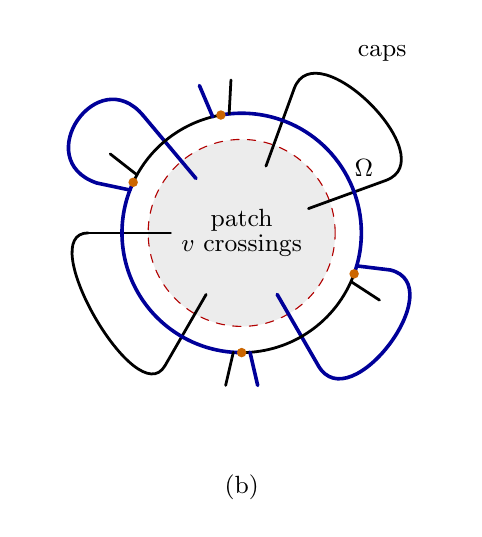
\begin{tikzpicture}[scale=0.95,line cap=round]
  \fill[gray!15] (0,0) circle[radius=1.25];
  \node[font=\small,align=center] at (0,0) {patch\\[-2pt]$v$ crossings};
  \draw[red!70!black,dashed] (0,0) circle[radius=1.25];
  % ports: road at 20,70,180,240; river at 130,300
  \foreach \a in {20,70,180,240} \draw[line width=1pt] (\a:0.95)--(\a:2.05);
  \foreach \a in {130,300} \draw[blue!60!black,line width=1.3pt] (\a:0.95)--(\a:2.05);
  % protective cycle: river-colored over road ports, road-colored over river ports
  \draw[blue!60!black,line width=1.3pt] (-20:1.6) arc[start angle=-20,end angle=100,radius=1.6];
  \draw[line width=1pt] (100:1.6) arc[start angle=100,end angle=155,radius=1.6];
  \draw[blue!60!black,line width=1.3pt] (155:1.6) arc[start angle=155,end angle=270,radius=1.6];
  \draw[line width=1pt] (270:1.6) arc[start angle=270,end angle=340,radius=1.6];
  % switch stubs, one of each color
  \foreach \a in {100,155,270,340}{
    \draw[line width=1pt] (\a-4:1.6)--(\a-6:2.05);
    \draw[blue!60!black,line width=1.3pt] (\a+4:1.6)--(\a+6:2.05);
    \fill[orange!80!black] (\a:1.6) circle[radius=1.8pt];
  }
  % schematic caps outside
  \draw[line width=1pt] (20:2.05) .. controls (20:2.9) and (70:2.9) .. (70:2.05);
  \draw[blue!60!black,line width=1.3pt] (130:2.05) .. controls (130:3.0) and (161:3.0) .. (161:2.05);
  \draw[line width=1pt] (180:2.05) .. controls (180:2.8) and (240:2.8) .. (240:2.05);
  \draw[blue!60!black,line width=1.3pt] (300:2.05) .. controls (300:2.9) and (346:2.9) .. (346:2.05);
  \node[font=\small] at (52:3.05) {caps};
  \node[font=\small] at (28:1.85) {$\Omega$};
  \node[font=\small] at (0,-3.4) {(b)};
\end{tikzpicture}
\caption{(a) The meander of Figure~\ref{fig:cut} with a separator (dashed). Its ports, the
points where it crosses the river or the road, are circled. (b) Completion of one side, schematically:
the patch inside the separator, the protective cycle $\Omega$ just outside it (river-colored where it
crosses road strands, road-colored where it crosses river strands, switching color at the dots), and
caps outside that close each color into one curve. The caps shown are only indicative.}
\label{fig:separator}
\end{figure}

\subsection{The reverse inequality}\label{sec:reverse}

\begin{proposition}[reverse inequality]\label{prop:reverse}
There is a constant $B$ such that for every sufficiently large $N$
\[ M_N\;\le\;e^{B\sqrt N}\max M_aM_b, \]
the maximum over integers $a,b$ with $N\le a+b\le N+8W$ and $N/10\le a,b\le 9N/10$, where
$W=\lceil4\sqrt{27N}\rceil$.
\end{proposition}

\begin{proof}[Key idea]
Choose, for each meander of order $N$, one separator as in Proposition~\ref{prop:noose}, with
$w\le W$ ports, and complete both sides as in Proposition~\ref{prop:disc}. The sides have $v_1+v_2=2N$
crossings with $N/2\le v_i\le3N/2$, and the completed meanders have orders $a$, $b$ with
$v_i/2\le a,b\le v_i/2+4w$. The original meander is recovered from the two completed meanders with
one marked crossing each, their two records, and the way the two boundary circles are glued, which
is an orientation and a rotation, at most $2w$ choices. The marks, the sizes, and the choice of which
crossing of the glued map is crossing $1$ of the original meander, and in which direction the river
runs, cost only a fixed polynomial in $N$. So the number of meanders of order $N$ is at
most a polynomial in $N$ times $e^{2c_\Omega W}$ times $\max M_aM_b$, and the polynomial is absorbed into
$e^{B\sqrt N}$. The ranges of $a$, $b$ follow from those of $v_i$ for large $N$.
\end{proof}

No ratio bound is used: the sizes $a$ and $b$ are allowed to exceed $N$ in total by $O(\sqrt N)$, and
that excess is handled in the next step by $\mu\le16$.

\subsection{The descending chain}\label{sec:descent}

\begin{proof}[Proof of the lower bound in Theorem~\ref{thm:main}]
By Proposition~\ref{prop:reverse}, for every large $N$ there are $a,b\in[N/10,9N/10]$ with
\[ L(a)+L(b)\;\le\;L(N)+(a+b-N)\log\mu+B\sqrt N\;\le\;L(N)+B_1\sqrt N , \]
using $a+b-N\le8W$ and $\mu\le16$. Divide by $a+b\ge N$ and use $L(N)\ge0$: one of the two, call it
$k$ and call it a \emph{child} of $N$, satisfies
\begin{equation}\label{eq:child}
\frac{L(k)}{k}\;\le\;\frac{L(N)}{N}+\frac{B_1}{\sqrt N}.
\end{equation}
Intuitively, passing to a child increases the loss per crossing, $L(k)/k$, only slightly. Fix a large target $n$ and start
from a huge $N_0$. Pass repeatedly to a child, and stop at the first size $k\le n$; then
$n/10<k\le n$. Each step
shrinks the size by a factor between $1/10$ and $9/10$, so, read backward from the last one, the
sizes grow at least geometrically and the added terms $B_1/\sqrt{\text{size}}$ sum to at most a
constant times $1/\sqrt n$. Choosing $N_0$ so large that $L(N_0)/N_0\le1/\sqrt n$ gives a $k$ in
$(n/10,n]$ with $L(k)\le B_2\sqrt n$, for every large $n$.

Now take any $n$. Split off such a size $k_1\in(n/10,n]$, then such a size $k_2$ for the remainder
$n-k_1\le9n/10$, and so on. By subadditivity~\eqref{eq:subadd}, $L(n)$ is at most
$L(k_1)+L(k_2)+\cdots$ plus a bounded term for the last small remainder. Each $L(k_i)$ is at most
$B_2$ times the square root of a geometrically decreasing size, so the sum is at most a constant
times $\sqrt n$. This gives
$L(n)\le C\sqrt n$ for large $n$, and enlarging $C$ covers small $n$.
\end{proof}

The same descent turns a reverse inequality $M_N\le e^{O(N^\tau)}\max M_aM_b$, for a fixed
$0<\tau<1$, into $L(n)=O(n^\tau)$, provided that the maximum runs over sizes $a,b$ between two fixed
fractions of $N$ with $a+b-N=O(N^\tau)$. The excess $a+b-N$ costs $(a+b-N)\log\mu$ in the first
display of the proof, and under these conditions the geometric sums still converge. Both conditions
are needed: with the excess $8W$ of Proposition~\ref{prop:reverse}, which is of order $\sqrt N$, the
descent gives only $L(n)=O(\sqrt n)$, however small the factor $e^{O(N^\tau)}$ is. With the earlier
completion the loss was
of order $\sqrt N\log N$, which gave the previous bound. The argument also extends, with the same
square root, to systems of several closed roads weighted by a parameter for each road; we do not use
this here.
